% Beamer template
% Author: Ozgur Taylan TURAN
% Delft University of Technology

\documentclass[aspectratio=169]{beamer}
\usepackage{/Users/ozgurtaylanturan/Documents/TeXThemes/beamer/beamerthemetot}
% PACKAGES
\usepackage[english]{babel}
\usepackage{graphicx}
\usepackage{animate}
%\usepackage{calc}
\usepackage{calligra}
\usepackage[absolute,overlay]{textpos}
\usepackage[T1]{fontenc}
%\usefonttheme{serif}
\usefonttheme{professionalfonts}
\usepackage{amsmath}
\usepackage{palatino}
\usepackage{mathpazo}
\usepackage{graphicx}
%\usepackage{subfig}
\usepackage{tikz}
\usetikzlibrary{shapes,arrows}
\usepackage{xcolor}
\usepackage[T1]{fontenc}
%\usefonttheme{serif}
%\usepackage{titling}
\usepackage{graphicx}
%\usepackage{subfig}
%\usepackage{tikz}
%\usetikzlibrary{shapes,arrows}
\usepackage{mathtools}
    
% BIB SETTINGS
\usepackage[backend=bibtex,firstinits=true,maxnames=30,maxcitenames=20,url=false,style=authoryear]{biblatex}
\bibliography{../../../Mendeley/bibtex/CoffeeTalks}

\setlength\bibitemsep{0.3cm} % space between entries in the reference list
\renewcommand{\bibfont}{\normalfont\scriptsize}
\renewcommand{\cite}[1]{\footnote<.->[frame]{\fullcite{#1}}}
\setbeamertemplate{bibliography item}{}

\setbeamertemplate{navigation symbols}{} % remove navigation symbols


 % COVER PAGE INFO   
\newcommand{\mytitle}{\color{White}\huge{\textbf{Coffee Talk \#1}}}
\newcommand{\mysubtitle}{\color{Pink}\Large{\textbf{Transfering Knowledge Across Learning Processes}}}
\newcommand{\myauthor}{\color{White}\textcalligra{\LARGE Ozgur Taylan Turan}}
\newcommand{\authorlabel}{\small O.T. Turan}
\author{\authorlabel}


\begin{document}
% COVER PAGE
{
{
\def\beamer@entrycode{\vspace*{-\headheight}}
\setbeamertemplate{frametitle}[default][center]
\setbeamertemplate{navigation symbols}{}
\usebackgroundtemplate{
\includegraphics[width=\paperwidth,height=\paperheight]{cover/coverart.pdf}}

\begin{frame}[plain] 

\begin{minipage}{\textwidth}
	\centering{\mytitle} \\
	%\vspace{1cm}
	%\centering{\mysubtitle} \\
	\vspace{1cm}
	\centering{\color{White}November 15, 2021} \\
	\vspace{1cm}
	\centering{\myauthor}\\
\end{minipage}
\end{frame}
}

\setbeamercovered{transparent}
\setbeamertemplate{footline}{\usebeamertemplate*{minimal footline}}
\setbeamertemplate{headline}{\usebeamertemplate*{minimal headline}}
\def\beamer@entrycode{\vspace*{-\headheight}}
}
% MAIN
\setbeamercovered{transparent}


\begin{frame}
	\centering
	\mysubtitle\cite{Flennerhag2018}
	Conference paper at 2019 ICLR
\end{frame}

\begin{frame}{Why This Paper?}
	\centering
	\begin{minipage}{0.5\textwidth}
		\begin{itemize}
			\item Neil Lawrence
			\item Transfer learning - Meta Learning
		\end{itemize}	
	\end{minipage}%
	\begin{minipage}{0.5\textwidth}
	\end{minipage}
\end{frame}

\begin{frame}{Introduction}
	\centering
	\begin{minipage}{0.4\textwidth}
		\begin{block}{\color{White} Problem with Transfer Learning}
			\begin{itemize}
				\item Structural affinity of tasks
				\item Information loss?
			\end{itemize}	
		\end{block}
	\end{minipage}% 
	\hspace{1cm} $\Longrightarrow$ \hspace{1cm}
	\begin{minipage}{0.4\textwidth}
		\begin{block}{\color{White}Solution with Meta Learning}
			\begin{itemize}
				\item Save relevant information 
				\item Aggregate task geometry info.
			\end{itemize}	
		\end{block}
	\end{minipage}
\end{frame}

\begin{frame}{Meta Learning}
	\begin{minipage}{0.5\textwidth}
		\begin{itemize}
			\item Learning a new task as a learning problem
			\item \color{Pink}BackProp entire learning process
		\end{itemize}	
	\end{minipage}%
	\begin{minipage}{0.5\textwidth}
	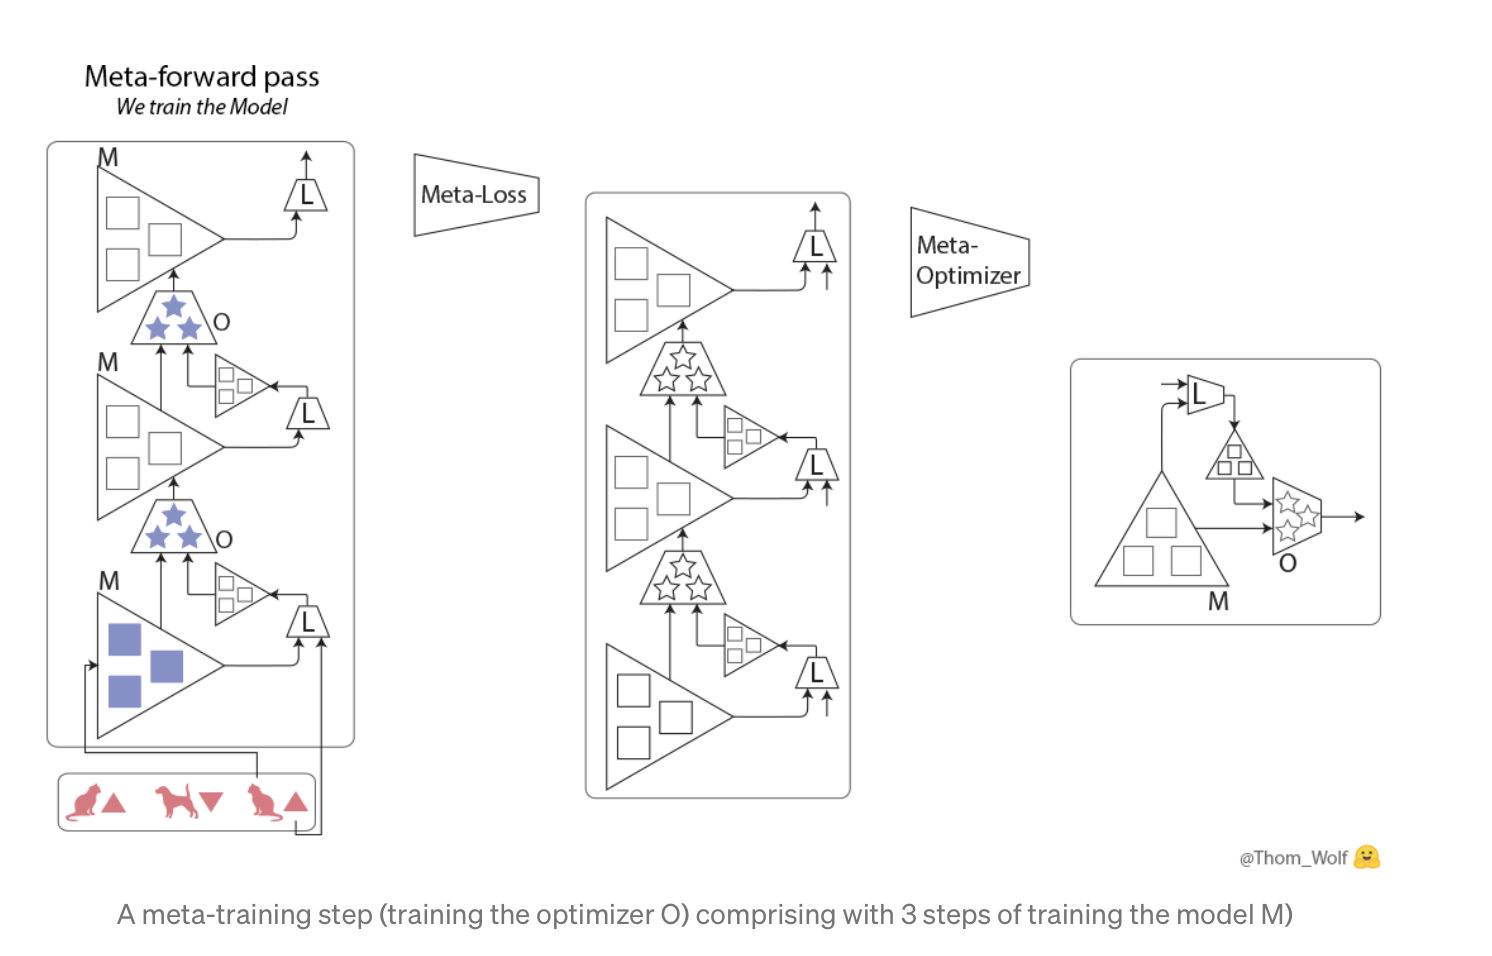
\includegraphics[width=1\textwidth]{Figures/meta}\cite{https://medium.com/huggingface/from-zero-to-research-an-introduction-to-meta-learning-8e16e677f78a}	
	\end{minipage}
\end{frame}

\begin{frame}{Loss Manifold}
	\begin{minipage}{0.40\textwidth}
		\begin{block}{\color{White}\# of Updates $\uparrow$}
		\begin{itemize}
			\item Loss manifold importance $\uparrow$
		\end{itemize}
		\end{block}
		\begin{block}{\color{White}Ease of Learning}
			\begin{itemize}
				\item Easier to navigate loss manif.
			\end{itemize}
		\end{block}
	\end{minipage}%
		\hspace{1cm}
	\begin{minipage}{0.5\textwidth}
		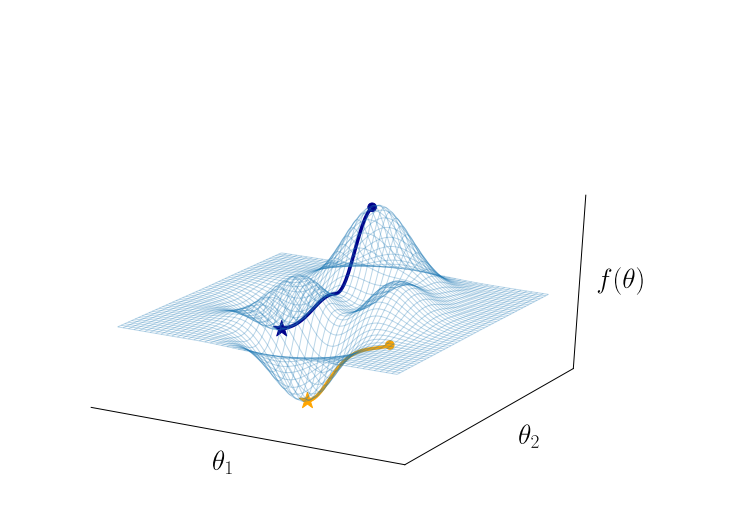
\includegraphics[width=\textwidth]{Figures/loss}
	\end{minipage}
\end{frame}

\begin{frame}{Leap}
	\begin{minipage}{0.45\textwidth}
		\begin{itemize}
			\item Framework that exploits geometry
			\item \color{Pink}Focus: \color{Black}point of initialization
			\item Learning and initialization relation
		\end{itemize}
		\begin{block}{\color{White}Learning Objective $f:\theta\in\mathbb{R}^n \to L  $}	
			$\theta^{i+1} = \theta^i -\alpha^i S^i\nabla f(\theta^i)$
		\end{block}
		\color{Pink}Assume convergence after K steps	
	\end{minipage}%
	\hspace{0.5cm}
	\begin{minipage}{0.5\textwidth}
		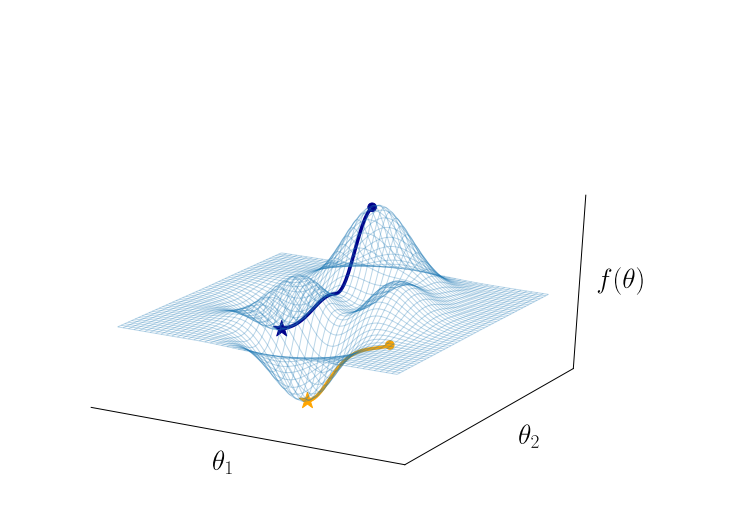
\includegraphics[width=\textwidth]{Figures/loss}
	\end{minipage}
\end{frame}



\begin{frame}{Meta objective}
	\begin{minipage}{0.5\textwidth}
	\begin{align*}
	\centering
	\min_{(\theta^0)} \quad & \mathbb{E}_{\tau}[d(\theta^0;M_\tau)] \\
		\text{s.t.} \quad  & \theta_\tau^{(i+1)}=u(\theta_\tau^i), \quad \theta_\tau^0=\theta^0, \\
		& \theta^0 \in \boldsymbol{\Theta}=\cap_\tau\{\theta^0 | f_\tau(\theta_\tau^{K_\tau}) \leq f_\tau(\psi_\tau^{K_\tau})\}
	\end{align*}
	\end{minipage}%
	\begin{minipage}{0.5\textwidth}
		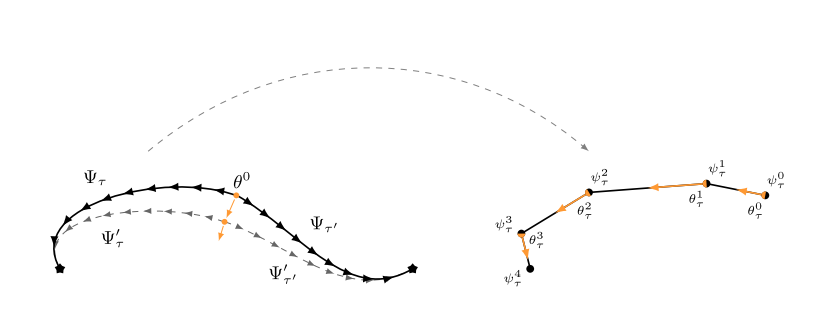
\includegraphics[width=\textwidth]{Figures/path}
	\end{minipage}
	\\
	\vspace{1cm}
		\centering
		\color{Pink} Minimize the expected learning path for all the tasks at the same time
\end{frame}

\begin{frame}{Results-[Omniglot]}
	\centering
	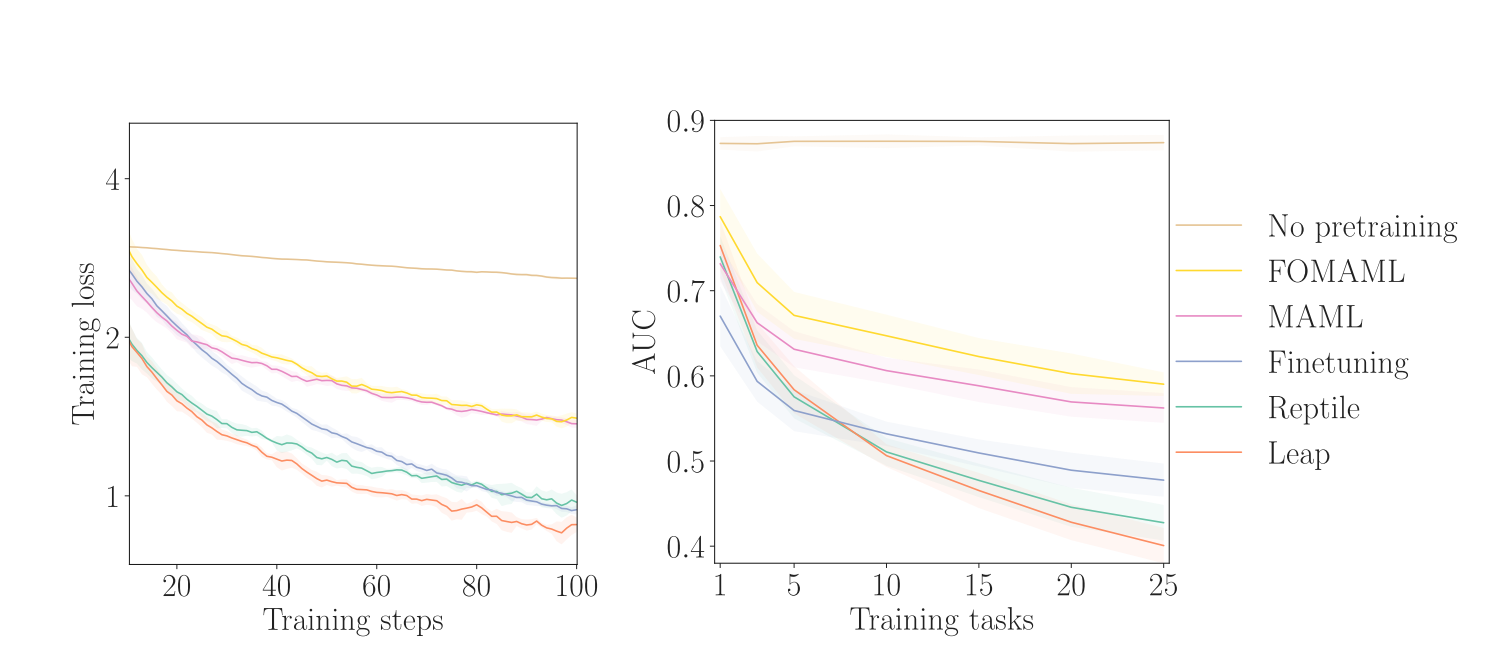
\includegraphics[width=0.8\textwidth]{Figures/omni}
	
	\color{Pink} Omniglot: dataset $\to$ 50 distinct alphabets show 1-25 and held 10 back
\end{frame}

\begin{frame}{Results-[Multi-CV]}
	\centering
	\begin{minipage}{0.5\textwidth}
		\color{Pink} Train for all and held-out one	
	\end{minipage}%
	\begin{minipage}{0.4\textwidth}
		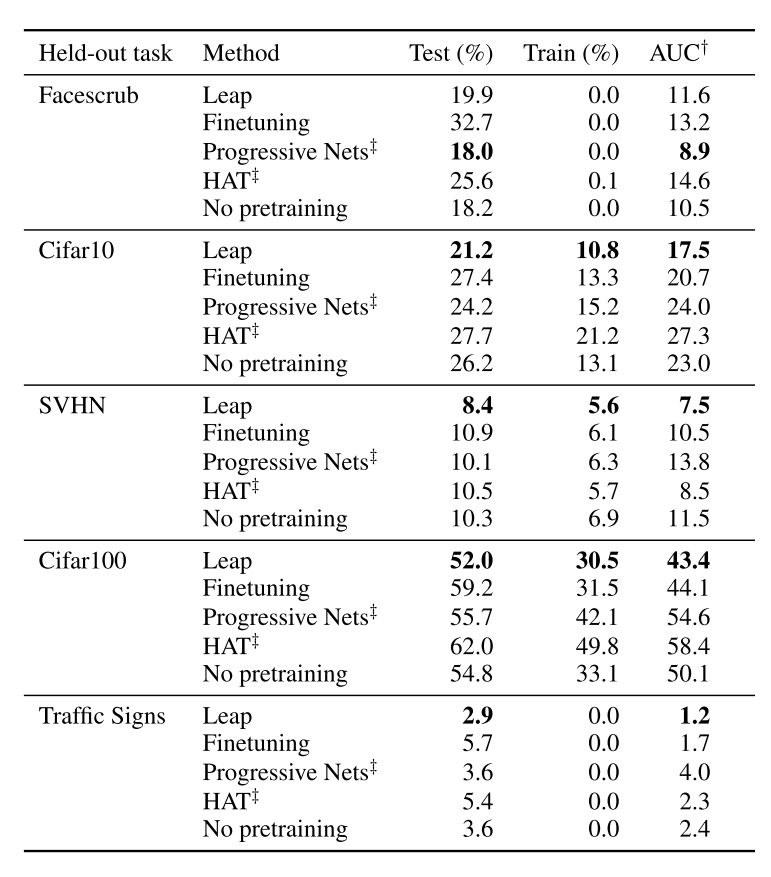
\includegraphics[width=1.0\textwidth]{Figures/multicv}
	\end{minipage}

\end{frame}

\begin{frame}
	\centering
	\color{Pink} Thanks for your attention!
\end{frame}






\end{document}